\chapter{Расчет потокораспределения и напряжений в узлах сети в послеаварийном режиме}
\label{cha:50-emergency}

Поскольку в послеаварийном режиме одна цепь линии ИП-ПС отключена, пересчитаем активное и индуктивное сопротивления линии ИП-ПС:
\[R_\textup{ИП-ПС} = \frac{R_0\cdot L_\textup{ИП-ПС}}{n_\textup{ц\, ИП-ПС}} = \frac{0,204\cdot 84}{1} = 17,1\; \text{Ом}\]
\[X_\textup{ИП-ПС} = \frac{X_0\cdot L_\textup{ИП-ПС}}{n_\textup{ц\, ИП-ПС}} = \frac{0,416\cdot 84}{1} = 34,9\; \text{Ом}\]

\section{Расчет нагрузок на шинах низшего и среднего напряжений подстанции}

Возьмем значения активной мощности на шинах низшего и среднего напряжений, $tg\varphi_\textup{н}$ и $cos\varphi_\textup{с}$ из табл. \ref*{tab:tabl2}.

Активная нагрузка на шинах низшего напряжения: $P_\textup{н} = 22,9 \; \text{МВт}$

Реактивная нагрузка на шинах НН вычисляется по формуле:
\begin{eqndesc}
	\begin{equation*}
		Q_\textup{н} = P_\textup{н}\cdot tg\varphi_\textup{н} = 22,9\cdot 0,44 = 10,1\; \text{МВар},
	\end{equation*}
	
	где $P_\textup{н}$ "--- активная нагрузка на шинах НН, \\
	$tg_{\varphi_{\text{н}}}$ "--- коэффициент реактивной мощности.
\end{eqndesc}

Активная нагрузка на шинах среднего напряжения (СН): $P_\textup{с} = 33\; \text{МВт}$

Реактивная нагрузка на шинах СН:
\begin{eqndesc}
	\begin{equation*}
		Q_\textup{с} = \sqrt{S_c^2 - P_c^2} = \sqrt{\left(\frac{P_c}{cos\varphi_c}\right)^2 - P_c^2} = \sqrt{\left(\frac{33}{0,82}\right)^2 - 33^2} = 23,0\; \text{Мвар},
	\end{equation*}
	
	где $P_\textup{с}$ "--- активная мощность нагрузки на шинах СН, \\
	$cos_{\varphi_{\text{с}}}$ "--- коэффициент мощности нагрузки, \\
	$S_\textup{с}$ "--- полная мощность на шинах СН.
\end{eqndesc}

\section{Расчет послеаварийного режима}
\textbf{1 этап}

Расчет первого этапа до определения зарядной мощности идентичен разделу \ref{cha:30-high_loads}.

Зарядная мощность в конце линии ИП-ПС уменьшиться в два раза, т.к. $n_\textup{ц}=1$:
\[\frac{Q_\textup{с.ИП-ПС}^{''}}{2} = \frac{1}{2}\cdot \frac{U_\textup{ном}^2\cdot B_\textup{л}}{2} = \frac{1}{2}\cdot \frac{110^2 \cdot 460,3\cdot 10^{-6}}{2} = 1,39\; \text{МВар} \]

Расчетная нагрузка подстанции:
\[S_p = S_\textup{прив} - j\frac{Q_\textup{с.ИП-ПС}^{''}}{2} = 56,2 + j40,4 - j1,39 = 56,2 + j39,0\; \text{МВА}\]

Мощность в конце линии ИП-ПС:
\[S_\textup{ИП-ПС}^{''} = S_p = 56,2 + j39,0\; \text{МВА}\]

Потери мощности в сопротивлении линии ИП:
\[\Delta S_\textup{ИП-ПС} = \frac{\left(S_\textup{ИП-ПС}^{''}\right)^2}{U_\textup{ном}^2}\cdot Z_\textup{л} = \frac{56,2^2 + 39,0^2}{110^2} \cdot (17,1 + j34,9) = 6,61 + j13,5 \; \text{МВА}\]

Мощность в начале линии ИП-ПС:
\[S_\textup{ИП-ПС}^{'} = S_\textup{ИП-ПС}^{''} + \Delta S_\textup{ИП-ПС} = 56,2 + j39,0 + 6,61 + j13,5 = 62,8 + j52,5\; \text{МВА}\]

Зарядная мощность в начале линии ИП-ПС уменьшится в два раза, т.к. $n_\textup{ц}=1$:
\[\frac{Q_\textup{с.ИП-ПС}^{'}}{2} = \frac{1}{2}\cdot \frac{U_\textup{ИП-ПС}^2\cdot B_\textup{л}}{2} = \frac{1}{2}\cdot \frac{124,3^2 \cdot 460,3\cdot 10^{-6}}{2} = 1,78\; \text{МВар}\]

Мощность, выдаваемая источником в сеть:
\[S_\textup{ИП-ПС} = S_\textup{ИП-ПС}^{'} - j\frac{Q_\textup{с.ИП-ПС}^{'}}{2} = 62,8 + j52,5 - j1,78 = 62,8 + j50,7\; \text{МВА}\]

\newpage

\textbf{2 этап}

%Продольная составляющая вектора падения напряжения находится по формуле:
%
%\begin{equation}
%	\Delta U_{12} = \frac{P_{12}^{(')('')}\cdot R_{12} + Q_{12}^{(')('')}\cdot X_{12}}{U_{(1)(2)}}
%\end{equation}
%
%Поперечной составляющей можем пренебречь, так как у нас линия уровня напряжения 110 кВ.
%
Продольная составляющая вектора падения напряжения на сопротивлении линии ИП-ПС:
\[\Delta U_\textup{ИП-ПС} = \frac{P_\textup{ИП-ПС}^{'}\cdot R_\textup{л} + Q_\textup{ИП-ПС}^{'}\cdot X_\textup{л}}{U_\textup{ИП-ПС}} = \frac{62,8\cdot 17,1 + 52,5\cdot 34,9}{124,3} = 23,4\; \text{кВ}\]

Напряжение на шинах ВН:
\[U_\textup{в} = U_\textup{ИП-ПС} - \Delta U_\textup{ИП-ПС} = 124,3 - 23,4 = 100,9 \; \text{кВ}\]

Продольная составляющая вектора падения напряжения на сопротивлении луча высшего напряжения:
\[\Delta U_\textup{в} = \frac{P_\textup{в}^{'}\cdot R_\textup{т.в} + Q_\textup{в}^{'}\cdot X_\textup{т.в}}{U_\textup{в}} = \frac{56,1\cdot 0,413 + 39,9\cdot 17,9}{100,9} = 7,31\; \text{кВ}\]

Напряжение в средней точке схемы замещения трансформаторов:
\[U_\textup{0} = U_\textup{в} - \Delta U_\textup{в} = 100,9 - 7,31 = 93,6 \; \text{кВ}\]

Продольная составляющая вектора падения напряжения на сопротивлении луча среднего напряжения:
\[\Delta U_\textup{с} = \frac{P_\textup{с}^{'}\cdot R_\textup{т.с} + Q_\textup{с}^{'}\cdot X_\textup{т.с}}{U_\textup{0}} = \frac{33,1\cdot 0,413 + 23,0\cdot 0}{93,6} = 0,146\; \text{кВ}\]

Напряжение на шинах СН, приведенное к стороне ВН:
\[U_\textup{с}^{'} = U_\textup{0} - \Delta U_\textup{н} = 93,6 - 0,146 = 93,5 \; \text{кВ}\]

Продольная составляющая вектора падения напряжения на сопротивлении луча низшего напряжения:
\[\Delta U_\textup{н} = \frac{P_\textup{н}^{'}\cdot R_\textup{т.н} + Q_\textup{н}^{'}\cdot X_\textup{т.н}}{U_\textup{0}} = \frac{22,9\cdot 0,413 + 10,6\cdot 10,3}{93,6} = 1,27\; \text{кВ}\]

Напряжение на шинах НН, приведенное к стороне ВН:
\[U_\textup{н} = U_\textup{0} - \Delta U_\textup{н} = 93,6 - 1,27 = 92,3 \; \text{кВ}\]

Полная расчетная схема замещения сети в послеаварийном режиме показана на рис. \ref{fig:rezhim_emergency}

\begin{sidewaysfigure}
	\centering
	\includegraphics[width=0.9\textwidth]{inc/svg/rezhim_emergency}
	\caption{Полная схема замещения сети в послеаварийном режиме}
	\label{fig:rezhim_emergency}
\end{sidewaysfigure}
